\section{Quantization Config Manager}
\label{sec:search}

In this section, we describe \qcm's search space of quantization configurations and its efficient search algorithm. Unlike checkpoint compression systems that use a predefined quantization configuration throughout training, the manager dynamically searches for a configuration that maximizes compression ratio while satisfying the quality constraint $\epsilon$ at every checkpoint.







\noindent\textbf{Search Space.} \autoref{tab:dq-search-space} describes the quantization configurations that comprise the search space of \qcm. To keep the search space manageable, we choose to use the same number of quantization bins across all layers except embedding layers. We use separate quantization parameters for embedding layers, since we have observed that embedding layers are considerably more sensitive to quantization, in line with findings from other research on Transformer model quantization \cite{gobo, Qbert}.





\begin{table}[h]
\centering
\begin{tabular}{@{\hspace{0px}} l l @{\hspace{0px}}}\\
\toprule
Parameter & Values \\
\midrule
Number of bins & 4, 6, 8, 12, 16, 32 \\
Pruning Fraction & 0, 0.1, 0.2, 0.3, 0.4, 0.5 \\
Pruning Metric & Magnitude, Sensitivity \\
Protection Fraction & 0.0005, 0.005, 0.01 \\
\bottomrule
\end{tabular}
\vspace{0.5em}
\caption{\small \sys's quantization configuration space.}
\label{tab:dq-search-space}
\end{table}


\noindent\textbf{Overview of the Search Algorithm.} Na\"ively evaluating each configuration in the search space is costly -- the search space contains over 200 configurations for non-embedding layers alone. To speed up the search, our key insight is that the optimal quantization configuration remains largely similar between adjacent checkpoints. At the first checkpoint, we perform a guided exhaustive search to identify the optimal configuration. Subsequently, we greedily evaluate the configurations that are close to the previous best configuration and only fall back to the exhaustive search if we can not identify a configuration that satisfies the quality constraint.  We observe that we need to resort to exhaustive search at most 2-3 times during model training. 



\begin{algorithm}[t]
\small
\caption{Guided Exhaustive Search}
\begin{algorithmic}[1]
\REQUIRE Quality threshold $T$, Configuration cube $C_{\text{cube}}$, Compression Ratio $CR_{\text{max}}$
\ENSURE Optimal configuration $C_{\text{opt}}$

\STATE $C_{\text{opt}} \gets \text{Null}$
\STATE $CR_{\text{max}} \gets 0$

\STATE $Diagonal \gets \text{GetDiagonal}(C_{\text{cube}})$
\STATE $C_{\text{opt}}, CR_{\text{max}} \gets \text{ParallelSearch}(Diagonal, T)$
\STATE $SubCubes \gets \text{GetFeasibleSubCubes}(C_{\text{cube}}, C_{\text{opt}})$
\FOR {each $SubCube$ in $SubCubes$}
\STATE $C_{\text{temp}}, CR_{\text{temp}} \gets \text{GuidedExhaustiveSearch}(T, SubCube)$
\IF{$CR_{\text{temp}} > CR_{\text{max}}$}
\STATE $C_{\text{opt}} \gets C_{\text{temp}}$
\STATE $CR_{\text{max}} \gets CR_{\text{temp}}$
\ENDIF
\ENDFOR
\RETURN $C_{\text{opt}}$
\end{algorithmic}\label{algo:guided-search}
\end{algorithm}


\noindent\textbf{Guided Exhaustive Search.} We use domain knowledge to reduce the cost of exhaustive search. If there was only one parameter, like the number of quantization bins, model quality would increase monotonically with the number of bins, while the compression ratio decreases. In this setting, we can find the optimal number of bins using a variation of binary search. We apply this approach to multiple configuration parameters, organizing them in a `configuration cube' where each axis represents a configuration knob as shown in \cref{fig:config-cube}. This layout ensures a monotonic increase in model quality across each axis, allowing us to use a divide-and-conquer method (\cref{algo:guided-search}). We repeat this search procedure with the two pruning metrics, magnitude and sensitivity, and select the better of the two.


\begin{figure}
    \centering
    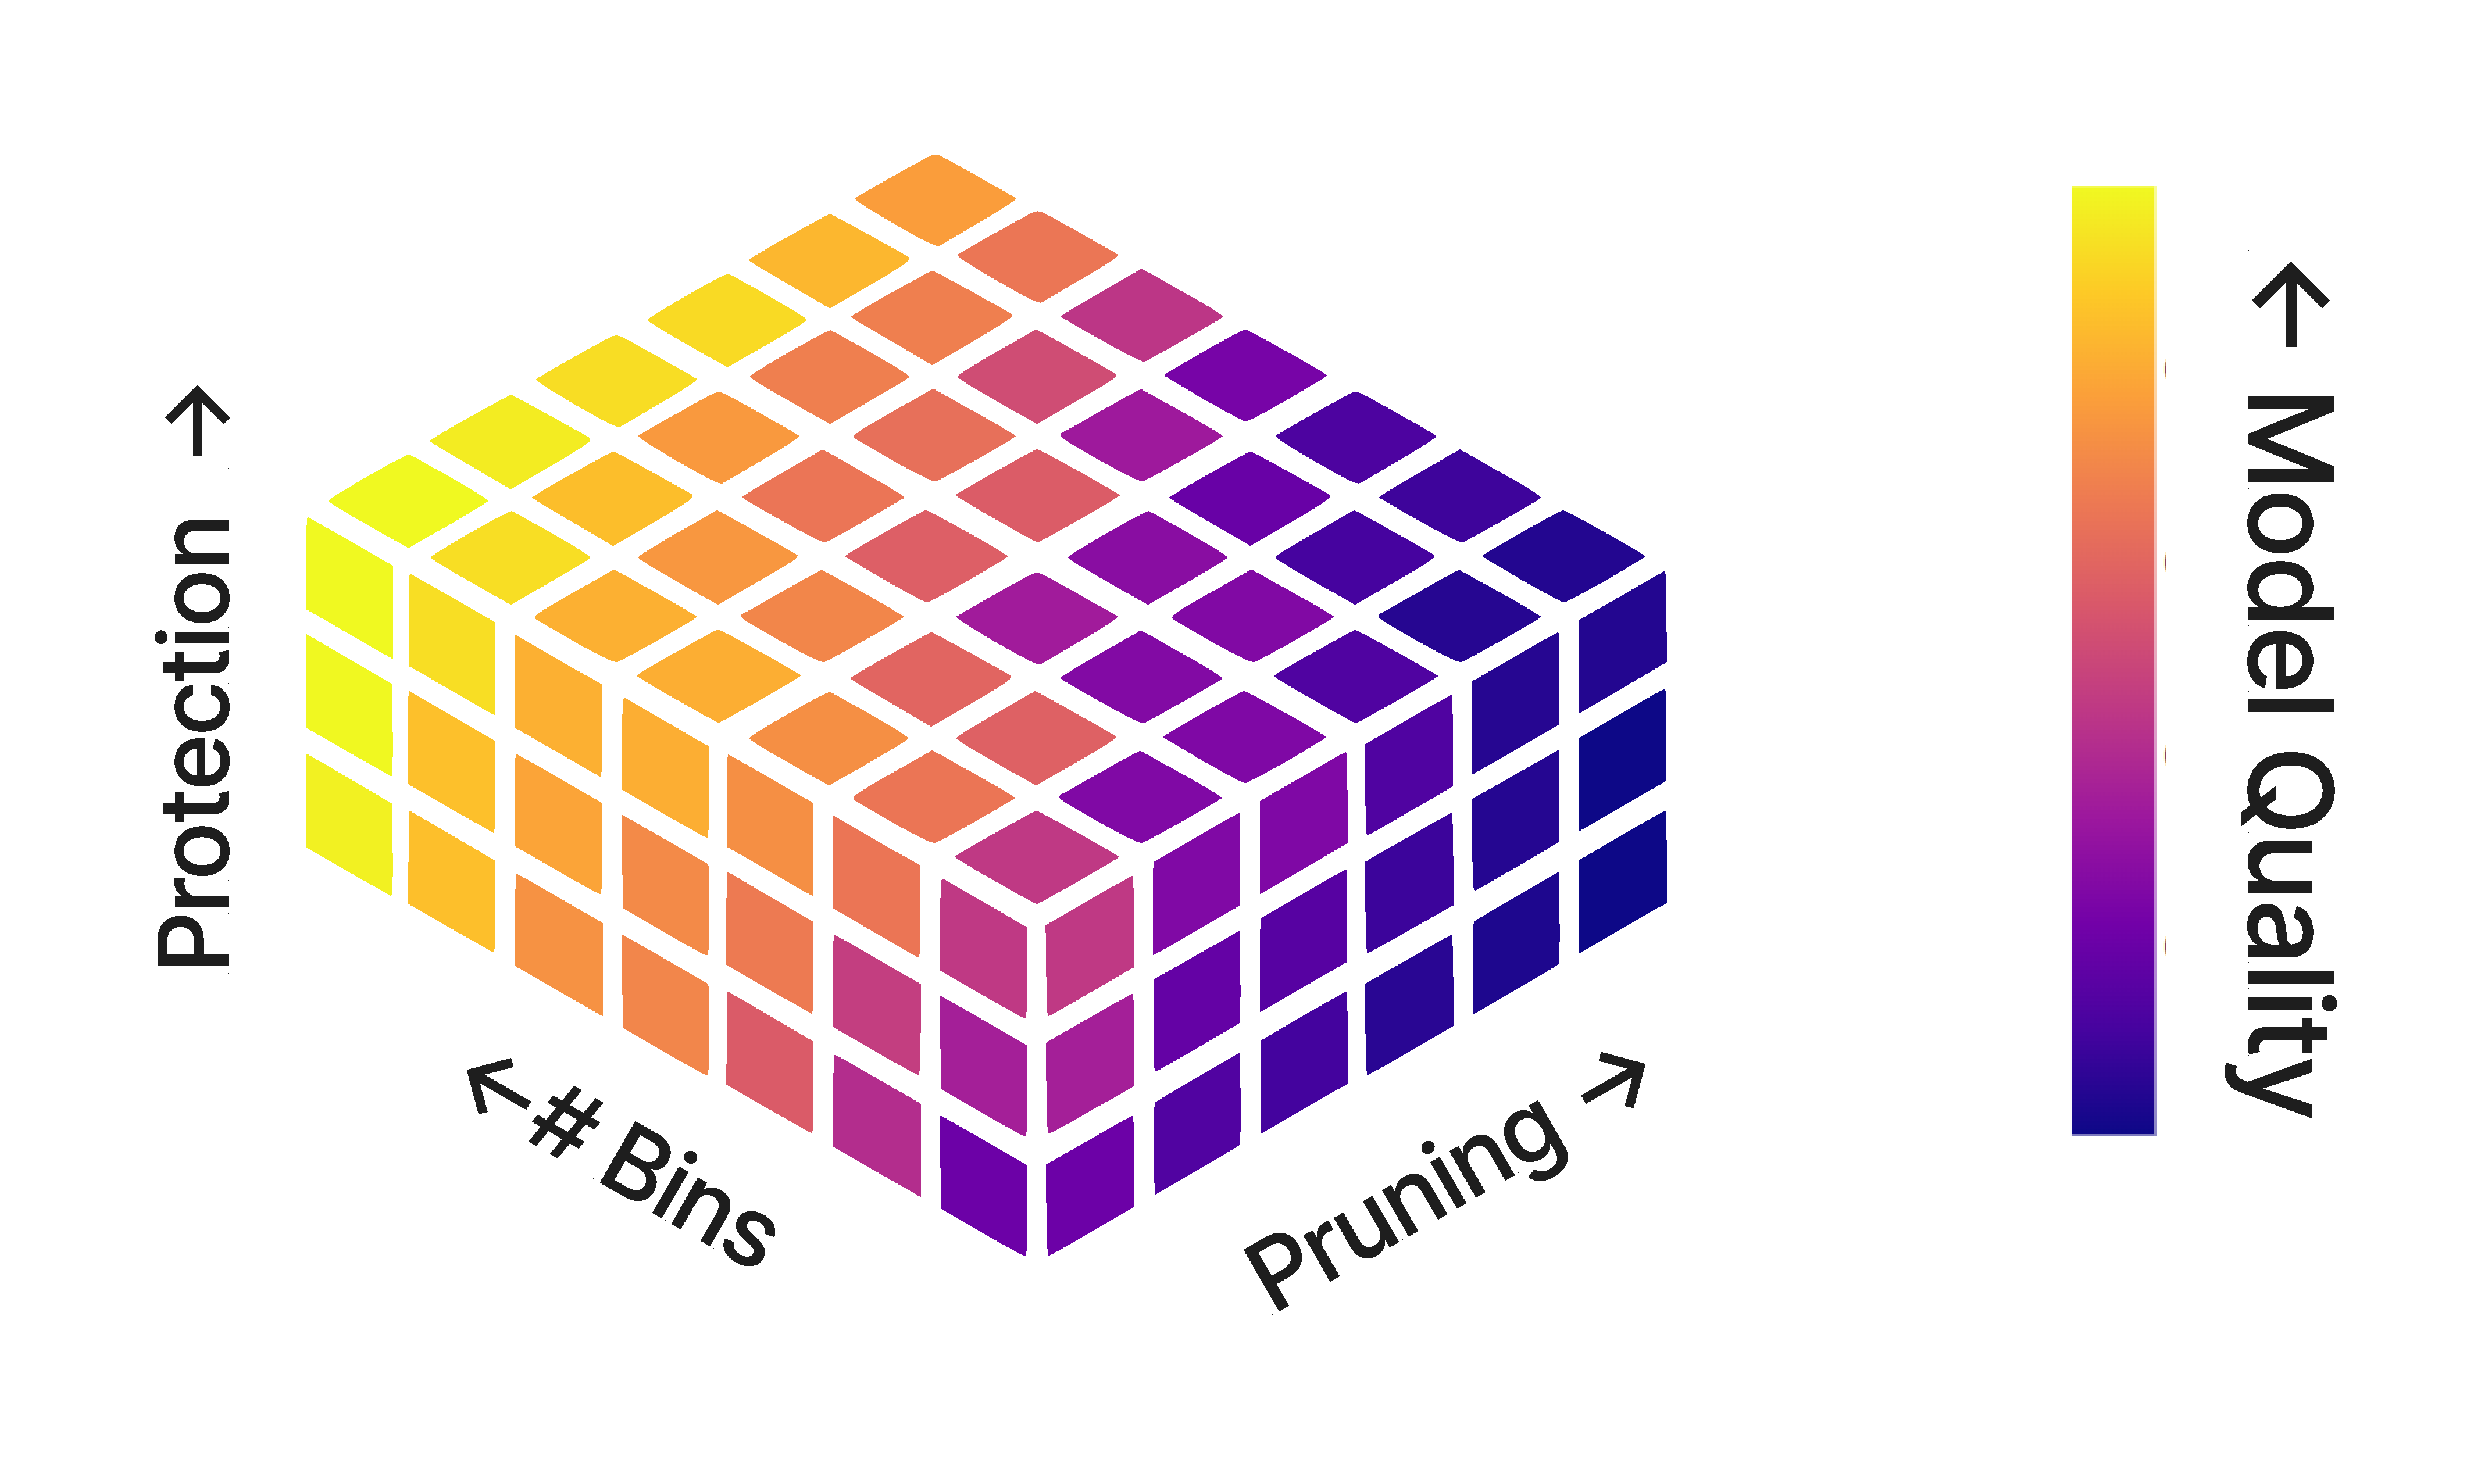
\includegraphics[width=0.75\linewidth]{figures/solution/config_cube_large_img.pdf}
    \caption{\small 
        Configuration search space as a function of pruning fraction, protection fraction, and number of bins. The color gradient indicates the direction of higher quality.%
    }
    \vspace{-1em}
    \label{fig:config-cube}
\end{figure}


\noindent\textbf{Delta-Neighbourhood Search.} In the steady-state, we obtain a suitable configuration by greedily selecting the best configuration within the $e$-delta neighborhood of the configuration chosen at the previous checkpoint. The $e$-delta neighborhood is defined as all configurations that are at most $e$ steps away in the configuration cube from the given configuration. At the start of each neighborhood search, we evaluate a configuration identical to the last best configuration, except with a different pruning metric. If we observe a significant improvement in the quantized model’s quality, we change the pruning metric and proceed with the neighborhood search using the new metric. As training progresses, the model becomes denser and more sensitive to compression. Hence, subsequent neighborhood searches intentionally rule out configurations more aggressive than the prior setting.




\noindent\textbf{Parallelized Implementation.} Since each data parallel replica maintains an identical model state, we can parallelize the search process. Configuration search trials are evaluated in groups of $m$, where $m$ is the degree of data parallelism. While scheduling the trials, we arrange them in a way that allows for an early exit. For instance, in the delta neighborhood search, we order the configurations in decreasing order of compression ratio. If in a given round of evaluation, we find a solution that satisfies the quality constraint, we can exit the search without evaluating the rest of the configurations. Our experiments show that for a data parallelism degree of eight, a high-quality configuration can be found within a single round of evaluation. %

